\begin{tikzpicture}
  \begin{scope}[yshift=0\columnwidth]
    \begin{scope}[xshift=0\columnwidth]
      \node [mybox] (box) at (-0.225\columnwidth, 0) {a)};
      \node [mybox] (box) {
        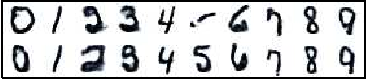
\includegraphics[width=0.4\columnwidth]{figures/rbm_samples}
      };
    \end{scope}
    \begin{scope}[xshift=0.5\columnwidth]
      \node [mybox] (box) at (-0.225\columnwidth, 0) {b)};
      \node [mybox] (box){
        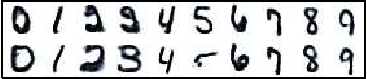
\includegraphics[width=0.4\columnwidth]{figures/rbm_witness_troughs}
      };
    \end{scope}
  \end{scope}
  \begin{scope}[yshift=-0.09\columnwidth]
    \begin{scope}[xshift=0\columnwidth]
      \node [mybox] (box) at (-0.225\columnwidth, 0) {c)};
      \node [mybox] (box) {
        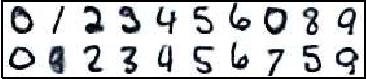
\includegraphics[width=0.4\columnwidth]{figures/many_rbm_cond_witness_troughs}
      };
    \end{scope}
    \begin{scope}[xshift=0.5\columnwidth]
      \node [mybox] (box) at (-0.225\columnwidth, 0) {d)};
      \node [mybox] (box){
        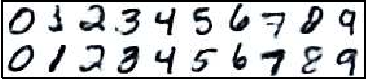
\includegraphics[width=0.4\columnwidth]{figures/dbn_ft_cond_witness_troughs}
      };
    \end{scope}
  \end{scope}
  \begin{scope}[yshift=-0.18\columnwidth]
    \begin{scope}[xshift=0\columnwidth]
      \node [mybox] (box) at (-0.225\columnwidth, 0) {e)};
      \node [mybox] (box) {
        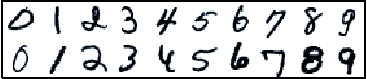
\includegraphics[width=0.4\columnwidth]{figures/many_rbm_cond_witness_peaks}
      };
    \end{scope}
    \begin{scope}[xshift=0.5\columnwidth]
      \node [mybox] (box) at (-0.225\columnwidth, 0) {f)};
      \node [mybox] (box){
        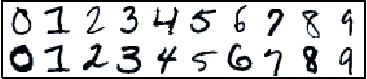
\includegraphics[width=0.4\columnwidth]{figures/dbn_ft_cond_witness_peaks}
      };
    \end{scope}
  \end{scope}
\end{tikzpicture}
% \begin{tabular}{cc}
%   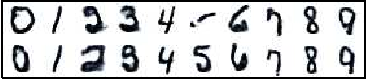
\includegraphics[width=0.45\columnwidth]{figures/rbm_samples} &
%   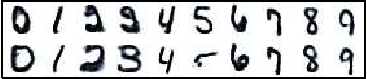
\includegraphics[width=0.45\columnwidth]{figures/rbm_witness_troughs}
%   \\
%   a) & b) \\
%   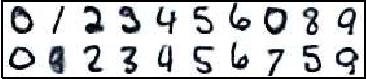
\includegraphics[width=0.45\columnwidth]{figures/many_rbm_cond_witness_troughs} &
%   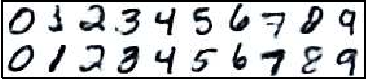
\includegraphics[width=0.45\columnwidth]{figures/dbn_ft_cond_witness_troughs}
%   \\
%   c) & d) \\
%   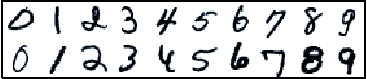
\includegraphics[width=0.45\columnwidth]{figures/many_rbm_cond_witness_peaks} &
%   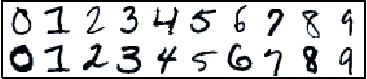
\includegraphics[width=0.45\columnwidth]{figures/dbn_ft_cond_witness_peaks}
%   \\
%   e) & f)
% \end{tabular}